% 第4章第1节：测试函数与广义函数（紧支撑测试、局部配对、广义函数的定义与例子、广义函数的微分）。

\section{测试函数与广义函数}
\label{sec:sob-distributions}

要把导数转移到另一个函数上，先得有一批足够好的“另一个函数”：它们要光滑，才能承受任意次求导；要在区域边界附近恒为零，才能让分部积分不留下边界项。本节先构造这样的测试函数，并说明一列测试“变得很小”应当怎样理解；然后把对测试的连续线性读数称为广义函数，看它怎样同时容纳局部可积函数、点读数和测度；最后定义广义函数的导数，并用$\delta_0$的导数说明这一新对象确实超出了函数和测度的范围。

这里要先说明一个名称。本节的对象在文献中传统上称为“分布”（distribution），与概率论中的概率分布毫无关系。为避免混淆，本书称它为广义函数，只在必要时提到“分布”这个旧称。

\subsection{测试函数与局部配对}
\label{sec:sob-test-functions}

\paragraph{光滑凸起}
我们先在实轴上造一个光滑、却在一个区间外恒为零的函数。关键的一块是$s\mapsto e^{-1/s}$（$s>0$），并在$s\le0$处补成零。它在$s>0$的各阶导数都形如$p_k(1/s)\,e^{-1/s}$，其中$p_k$是多项式，这可以对求导次数归纳验证；由于对任意$m$都有$s^{-m}e^{-1/s}\to0$（$s\to0^+$），每一阶导数从右侧趋于零，与左侧的零相接。于是这个函数在整条实轴上无穷次可微，却在$s\le0$上恒为零。代入$s=1-t^2$，得到
\begin{equation}
 \psi(t)=
 \begin{cases}
  \exp\!\left(-\dfrac{1}{1-t^2}\right), & |t|<1,\\[1ex]
  0, & |t|\ge1,
 \end{cases}
 \label{eq:sob-bump}
\end{equation}
它无穷次可微，在$(-1,1)$内为正，在$[-1,1]$外为零，最大值$\psi(0)=e^{-1}$。图~\ref{fig:sob-bump-cutoff}(a)画出了这个凸起。

\begin{figure}[!htb]
  \centering
  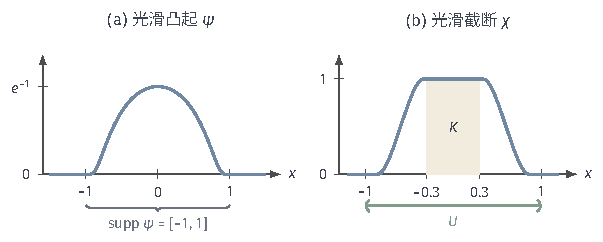
\includegraphics[width=102.2mm]{figures/02-abstract-mathematics/03-function-spaces/tikz/c4-bump-cutoff/figure.pdf}
  \caption{测试函数的两个基本构件。(a)~光滑凸起$\psi$，在$(-1,1)$内为正，在区间外恒为零，各阶导数在$\pm1$处都连续地接到零。(b)~光滑截断$\chi=\mathbf 1_{[-0.6,0.6]}*\rho_{0.3}$：在紧集$K=[-0.3,0.3]$（阴影）上恒为$1$，支撑$[-0.9,0.9]$落在开集$U=(-1,1)$内，中间光滑地由$1$降到$0$。}
  \label{fig:sob-bump-cutoff}
\end{figure}

在$\mathbb R^d$中，把$t^2$换成$|x|^2$就得到在单位开球内为正、在球外为零的光滑凸起$\psi(|x|)$，这里$|x|$是欧氏长度。平移伸缩为$\psi(|x-x_0|/r)$后，它的“非零区域”是以$x_0$为中心、半径为$r$的球。只要$r$小于$x_0$到$\Omega$边界的距离，这个凸起就整个待在$\Omega$内部，离边界还有一段间隔。

\paragraph{支撑与测试函数}
为了把“在边界附近恒为零”说准确，对函数$\varphi$定义它的\term{支撑}（support）
\[
 \operatorname{supp}\varphi=\overline{\{x:\varphi(x)\neq0\}},
\]
即非零点集合的闭包。记$C_c^\infty(\Omega)$为$\Omega$上无穷次可微、且支撑是$\Omega$的紧子集的函数全体，称其中的函数为\term{测试函数}（test function）。支撑紧含于$\Omega$，意味着它与边界保持正距离：存在$\delta>0$，使离边界不到$\delta$的点上$\varphi$恒为零。上面的平移凸起就是测试函数。

这一点立刻解决了分部积分的边界项。设$f\in C^1(\Omega)$，$\varphi\in C_c^\infty(\Omega)$。把$f\varphi$在$\Omega$外补成零，得到$\mathbb R^d$上紧支撑的$C^1$函数。沿第$j$个坐标方向的任一直线积分$\partial_j(f\varphi)$，由微积分基本定理得零，因为两端都落在支撑之外；再对其余坐标积分（Fubini定理~\ref{thm:analysis-fubini-integrable}），得到
\begin{equation}
 \int_\Omega(\partial_jf)\,\varphi\,\mathrm dx=-\int_\Omega f\,\partial_j\varphi\,\mathrm dx .
 \label{eq:sob-integration-by-parts}
\end{equation}
式~\eqref{eq:sob-integration-by-parts}没有边界项，并且右端已不再出现$f$的导数。本章后面的全部构造都从这个等式出发。

\paragraph{局部可积函数}
要让$\int_\Omega f\varphi\,\mathrm dx$有意义，$f$需要满足什么条件？测试函数只在一个紧集上非零，并且在那里有界，所以只需要$f$在每个紧集上可积。称可测函数$f$\term{局部可积}（locally integrable），若对每个紧集$K\subset\Omega$都有$\int_K|f|\,\mathrm dx<\infty$，记作$f\in L^1_{\mathrm{loc}}(\Omega)$；与$L^p$空间一样，几乎处处相等的函数视为同一元素。对$f\in L^1_{\mathrm{loc}}(\Omega)$和支撑在紧集$K$内的测试$\varphi$，
\begin{equation}
 \left|\int_\Omega f\varphi\,\mathrm dx\right|\le\left(\int_K|f|\,\mathrm dx\right)\sup_K|\varphi| ,
 \label{eq:sob-local-pairing}
\end{equation}
右端有限，配对良好定义，而且改变$f$在一个零测集上的值不影响积分。

局部可积比可积宽得多，也依赖于区域。$f(x)=1/x$在$(0,1)$上局部可积：$(0,1)$的紧子集离$0$有正距离，$1/x$在其上有界；但$\int_0^1 x^{-1}\,\mathrm dx=\infty$，所以它不在$L^1(0,1)$中。把区域换成整条实轴，任何含原点的紧区间上积分都发散，$1/x$便不再局部可积。再看$\mathbb R^d$中的幂函数$|x|^{-a}$：按例~\ref{ex:region-power-function-threshold}的二进壳层估计，$d$维壳层$\{2^k\le|x|<2^{k+1}\}$的体积按$2^{kd}$缩放，于是单位球上$\int|x|^{-a}\,\mathrm dx<\infty$当且仅当$a<d$。因此$|x|^{-a}\in L^1_{\mathrm{loc}}(\mathbb R^d)$当且仅当$a<d$。这个阈值在后面检验弱导数和嵌入时会反复使用。

\paragraph{光滑截断}
后面经常需要这样一个测试：它在一个给定紧集上恒等于$1$，又不越出一个给定的开邻域。凸起$\psi$只在一点取最大值，不够用；把它归一化后与示性函数作局部平均，就能得到所需的平台。令$c_d=\int_{\mathbb R^d}\psi(|x|)\,\mathrm dx$，
\begin{equation}
 \rho(x)=c_d^{-1}\psi(|x|),\qquad \rho_\varepsilon(x)=\varepsilon^{-d}\rho(x/\varepsilon)\quad(\varepsilon>0).
 \label{eq:sob-mollifier}
\end{equation}
由换元，$\rho_\varepsilon$非负、光滑、积分为$1$，支撑是闭球$\overline{B}(0,\varepsilon)$。一维时$c_1\approx0.4440$。第~\ref{sec:sob-mollification}节还会把$\rho_\varepsilon$当作局部平均的权重系统使用。

\begin{lemma}[光滑截断]
\label{lem:sob-cutoff}
设$K\subset U\subset\Omega$，$K$紧，$U$开。则存在$\chi\in C_c^\infty(U)$，满足$0\le\chi\le1$，并在$K$上$\chi=1$。
\end{lemma}

\begin{proof}
取$\delta>0$，使$3\delta$小于$K$到$U$的补集的距离（$U=\mathbb R^d$时任取$\delta>0$）；紧集到不相交闭集的距离为正，所以这样的$\delta$存在。记$K_\delta=\{x:\operatorname{dist}(x,K)\le\delta\}$，令
\[
 \chi(x)=\int_{\mathbb R^d}\mathbf 1_{K_\delta}(y)\,\rho_\delta(x-y)\,\mathrm dy .
\]
被积函数对$x$的各阶导数为$\mathbf 1_{K_\delta}(y)D^\alpha\rho_\delta(x-y)$，绝对值不超过$\sup|D^\alpha\rho_\delta|\cdot\mathbf 1_{K_\delta}(y)$，后者与$x$无关且可积，因此可以在积分号下逐次求导（第~\ref{sec:multivariable-parameter-integrals}节），$\chi$无穷次可微。由于$\rho_\delta\ge0$且积分为$1$，有$0\le\chi\le1$。

若$x\in K$，则$\rho_\delta(x-\cdot)$的支撑$\overline B(x,\delta)\subset K_\delta$，积分等于$\int\rho_\delta=1$。若$\operatorname{dist}(x,K)>2\delta$，则$\overline B(x,\delta)$与$K_\delta$不交，$\chi(x)=0$。所以$\operatorname{supp}\chi\subset\{x:\operatorname{dist}(x,K)\le2\delta\}$，这是一个紧集，并且由$\delta$的取法含于$U$。
\end{proof}

图~\ref{fig:sob-bump-cutoff}(b)给出一维的例子：$K=[-0.3,0.3]$，$U=(-1,1)$，取$\delta=0.3$，$\chi=\mathbf 1_{[-0.6,0.6]}*\rho_{0.3}$在$K$上为$1$，在$[-0.9,0.9]$外为零。截断让我们能够“只看一块区域”而不引入跳跃，它在下一节证明测试函数能区分局部可积函数时起关键作用。

\paragraph{测试函数列怎样才算趋零}
广义函数将是测试上的线性读数，我们希望它对测试的小变化作出小反应。那么一列测试$\varphi_n$怎样才算“趋于零”？只看函数值的最大偏差是不够的。图~\ref{fig:sob-test-sequences}比较了三列测试，其中$\psi$为式~\eqref{eq:sob-bump}的凸起。

\begin{figure*}[!htb]
  \centering
  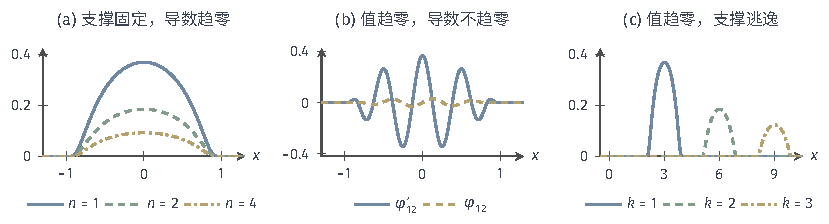
\includegraphics[width=140.4mm]{figures/02-abstract-mathematics/03-function-spaces/tikz/c4-test-sequences/figure.pdf}
  \caption{三列测试函数的对照。(a)~$\psi/n$：支撑固定在$[-1,1]$，函数值及各阶导数都一致趋零，这是测试意义下的趋零。(b)~$\varphi_n=\psi(x)\sin(nx)/n$，图中$n=12$：函数值（虚线）的上确界不超过$e^{-1}/12\approx0.031$，导数（实线）的上确界却约为$e^{-1}\approx0.37$，不随$n$减小。(c)~$\psi(x-3k)/k$：函数值和导数都一致趋零，支撑却跑向无穷远，不落在同一个紧集内。}
  \label{fig:sob-test-sequences}
\end{figure*}

第一列$\psi/n$的支撑固定，每一阶导数都是$D^\alpha\psi/n$，一致趋零；无论用什么合理的方式衡量，它都在变小。第二列$\varphi_n(x)=\psi(x)\sin(nx)/n$的函数值一致趋零，但
\[
 \varphi_n'(x)=\frac{\psi'(x)\sin(nx)}{n}+\psi(x)\cos(nx),
\]
第二项在原点等于$\psi(0)=e^{-1}$，导数并不变小。第三列$\psi(x-3k)/k$的函数值与各阶导数都一致趋零，但支撑向右逃逸，任何固定的紧集都装不下所有项。

后两列在测试意义下都不应算作趋零，因为确实存在合理的读数对它们给出不趋零的结果。读取原点导数的$\varphi\mapsto-\varphi'(0)$在第二列上恒为$-e^{-1}$；读数$\varphi\mapsto\sum_{k\ge1}k\,\varphi(3k)$在每个测试上只有有限项非零，因而有定义，它在第三列的第$k$项上取值$k\cdot\psi(0)/k=e^{-1}$。这两个读数都会在下面被确认为广义函数。于是测试的收敛必须同时控制支撑和所有阶导数：称$\varphi_n\to\varphi$（在测试意义下），若存在同一个紧集$K\subset\Omega$包含所有$\operatorname{supp}\varphi_n$与$\operatorname{supp}\varphi$，并且对每个多重指标$\alpha$都有$\sup_K|D^\alpha\varphi_n-D^\alpha\varphi|\to0$。这里的多重指标约定见第~\ref{sec:sob-distribution-derivative}节；在一维，$D^\alpha$就是$k$阶导数。

这一收敛不是由某一个范数给出的：上确界范数忽略导数，加入有限阶导数也挡不住更高阶的振荡，而支撑条件根本不是范数能表达的。完整的做法是在$C_c^\infty(\Omega)$上建立一种局部凸拓扑，本章不展开这一理论，只使用上面这个序列判据以及下一小节与之配套的估计。

\subsection{广义函数的定义与例子}
\label{sec:sob-distribution-def}

有了测试函数，我们把“对每个测试给出一个数”的对象作为新的研究对象。它应当是线性的，并且在每个固定的紧集上，读数受测试的有限阶导数的大小控制。

\begin{definition}[广义函数]
\label{def:sob-distribution}
称线性映射$T:C_c^\infty(\Omega)\to\mathbb F$为$\Omega$上的\term{广义函数}（generalized function，传统上称distribution），若对每个紧集$K\subset\Omega$，存在常数$C_K\ge0$和非负整数$m_K$，使所有支撑含于$K$的测试$\varphi$满足
\begin{equation}
 |T(\varphi)|\le C_K\sum_{|\alpha|\le m_K}\sup_K|D^\alpha\varphi| .
 \label{eq:sob-distribution-estimate}
\end{equation}
$\Omega$上广义函数的全体记作$\mathcal D'(\Omega)$。
\end{definition}

估计~\eqref{eq:sob-distribution-estimate}保证了上一小节要求的连续性：若$\varphi_n\to\varphi$（测试意义下），所有支撑落在同一个$K$内，对差$\varphi_n-\varphi$用这个估计，右端是有限多个一致趋零的量之和，所以$T(\varphi_n)\to T(\varphi)$。常数$C_K$与阶数$m_K$可以随紧集变化，这让广义函数在区域内部“越靠近边界越剧烈”也被允许。可以证明，反过来序列连续也推出这样的估计，因此两种说法等价；本章只用估计这一侧。广义函数作为线性泛函的观点，与第~\ref{sec:lfo-operators}节对有界线性泛函的讨论一致，区别在于这里的定义域$C_c^\infty(\Omega)$不是赋范空间，连续性只能逐个紧集表述。

\paragraph{由局部可积函数给出的广义函数}
对$f\in L^1_{\mathrm{loc}}(\Omega)$定义
\begin{equation}
 T_f(\varphi)=\int_\Omega f\varphi\,\mathrm dx .
 \label{eq:sob-regular-distribution}
\end{equation}
线性是显然的，估计~\eqref{eq:sob-local-pairing}正是$m_K=0$、$C_K=\int_K|f|$时的式~\eqref{eq:sob-distribution-estimate}，所以$T_f$是广义函数。几乎处处相等的$f$给出同一个$T_f$；下一节将证明反过来也成立，即$T_f=T_g$推出$f=g$几乎处处，于是可以把局部可积函数看作特殊的广义函数而不丢失信息。要强调的是，$T_f$读取的是$f$与测试的加权平均，并没有给$f$补上任何一点处的值：$1/x$在$(0,1)$上产生的广义函数，同样不回答“$f$在某点等于多少”。

\paragraph{点读数与测度}
不由普通函数给出的最简单例子是点读数。固定$x_0\in\Omega$，令
\[
 \delta_{x_0}(\varphi)=\varphi(x_0).
\]
它显然线性，并满足$|\delta_{x_0}(\varphi)|\le\sup_K|\varphi|$，取$m_K=0$、$C_K=1$即可，所以它是广义函数，称为\term{Dirac广义函数}（Dirac delta）。第~\ref{sec:sob-kinks-jumps}节将证明，不存在局部可积函数$g$使$\delta_{x_0}=T_g$。

点读数是测度积分的特例。设$\mu$是$\Omega$上的Borel测度，并且在每个紧集上取有限值（称为局部有限测度），令
\[
 T_\mu(\varphi)=\int_\Omega\varphi\,\mathrm d\mu ,\qquad |T_\mu(\varphi)|\le\mu(K)\sup_K|\varphi| .
\]
它也是$m_K=0$的广义函数。$\delta_{x_0}$对应集中在$x_0$的单位点质量，即第~\ref{sec:lfo-ck-dual}节的Dirac测度；上一小节的读数$\sum_{k\ge1}k\,\varphi(3k)$来自测度$\sum_kk\,\delta_{3k}$，每个紧集只含有限个质点，测度局部有限，所以它也是广义函数；$T_f$在$f\ge0$时对应以$f$为密度的测度$f\,\mathrm dx$，与第~\ref{sec:measure-same-space-comparison}节的Radon--Nikodym密度一致。允许测度带符号（在每个紧集上全变差有限）时，同样的估计以全变差$|\mu|(K)$代替$\mu(K)$。

这样，局部可积函数和局部有限测度都能产生广义函数，但广义函数比它们更宽。它不必是正的：若对所有非负测试都有$T(\varphi)\ge0$，称$T$为正的，$T_f$只在$f\ge0$几乎处处时才正。它也不必由测度给出：由测度给出的广义函数都满足$m_K=0$的估计，只受测试函数值的控制，而下一小节的$D\delta_0$需要读取测试的导数，将越出这一范围。

\subsection{广义函数的微分}
\label{sec:sob-distribution-derivative}

现在可以把导数转移到测试上。先约定多变量的记号。\term{多重指标}（multi-index）是非负整数组$\alpha=(\alpha_1,\ldots,\alpha_d)$，其阶数$|\alpha|=\alpha_1+\cdots+\alpha_d$，对应的偏导数
\[
 D^\alpha=\partial_1^{\alpha_1}\cdots\partial_d^{\alpha_d}.
\]
例如$d=2$、$\alpha=(1,2)$时，$D^\alpha=\partial_1\partial_2^2$，阶数为$3$；$\alpha=(0,\ldots,0)$时约定$D^\alpha$为恒等运算。测试函数的混合偏导数与求导次序无关，因此$D^\alpha$的定义没有歧义。

对$f\in C^{|\alpha|}(\Omega)$和测试$\varphi$，把式~\eqref{eq:sob-integration-by-parts}逐坐标重复$|\alpha|$次，每转移一次导数产生一个负号，测试的紧支撑使每一步都没有边界项：
\begin{equation}
 \int_\Omega(D^\alpha f)\,\varphi\,\mathrm dx=(-1)^{|\alpha|}\int_\Omega f\,D^\alpha\varphi\,\mathrm dx .
 \label{eq:sob-repeated-parts}
\end{equation}
用广义函数的语言，左端是$T_{D^\alpha f}(\varphi)$，右端是$(-1)^{|\alpha|}T_f(D^\alpha\varphi)$。右端对任何广义函数都有意义，于是取它作为定义。

\begin{definition}[广义导数]
\label{def:sob-distribution-derivative}
设$T\in\mathcal D'(\Omega)$，$\alpha$为多重指标。定义$T$的$\alpha$阶\term{广义导数}（distributional derivative）为
\begin{equation}
 (D^\alpha T)(\varphi)=(-1)^{|\alpha|}\,T(D^\alpha\varphi),\qquad\varphi\in C_c^\infty(\Omega).
 \label{eq:sob-distribution-derivative}
\end{equation}
\end{definition}

我们需要核对$D^\alpha T$仍是广义函数。线性由$T$和$D^\alpha$的线性得到。对支撑含于$K$的测试，$D^\alpha\varphi$的支撑也在$K$内，代入$T$的估计，
\[
 |(D^\alpha T)(\varphi)|\le C_K\sum_{|\beta|\le m_K}\sup_K|D^{\beta}D^\alpha\varphi|
 \le C_K\sum_{|\gamma|\le m_K+|\alpha|}\sup_K|D^\gamma\varphi| ,
\]
所以$D^\alpha T$满足阶数为$m_K+|\alpha|$的估计。由此得到三条基本性质。其一，每个广义函数都可以求任意阶导数，导数仍是广义函数，这与经典导数截然不同。其二，由式~\eqref{eq:sob-repeated-parts}，当$f\in C^{|\alpha|}(\Omega)$时$D^\alpha T_f=T_{D^\alpha f}$，新定义与经典导数相容。其三，因为测试的混合偏导数可交换，$D^\alpha D^\beta T=D^{\alpha+\beta}T$，广义导数的次序也无关紧要。

\paragraph{点读数的导数}
看最简单的非函数对象。在实轴上，按定义
\[
 (D\delta_0)(\varphi)=-\delta_0(\varphi')=-\varphi'(0).
\]
$D\delta_0$读取测试在原点的导数并反号，它满足$m_K=1$的估计$|(D\delta_0)(\varphi)|\le\sup_K|\varphi'|$。直观地说，$\delta_0$是集中在原点的单位质量，$D\delta_0$则像在原点两侧紧挨着放置一正一负两个质量所形成的“偶极子”。

$D\delta_0$不能由任何测度给出，下面用固定支撑、函数值有界而原点导数无界的测试来说明。

\begin{example}[$D\delta_0$不是测度]
\label{ex:sob-ddelta-not-measure}
设有实轴上的带符号Borel测度$\mu$，在紧集上全变差有限，并且$D\delta_0=T_\mu$。取光滑截断$\chi$，使其在$[-0.3,0.3]$上为$1$、支撑在$[-0.9,0.9]$内（例如图~\ref{fig:sob-bump-cutoff}(b)中的函数），令
\[
 \varphi_n(x)=\chi(x)\sin(nx).
\]
每个$\varphi_n$的支撑都在$K=[-0.9,0.9]$内，且$|\varphi_n|\le1$。由于$\chi$在原点附近恒为$1$，$\varphi_n'(0)=n\cos0=n$。一方面$|T_\mu(\varphi_n)|\le|\mu|(K)\sup|\varphi_n|\le|\mu|(K)$；另一方面$|(D\delta_0)(\varphi_n)|=|\varphi_n'(0)|=n$。令$n\to\infty$即得矛盾。图~\ref{fig:sob-ddelta-test}画出$n=3$与$n=10$的测试及其原点切线。
\end{example}

\begin{figure}[!htb]
  \centering
  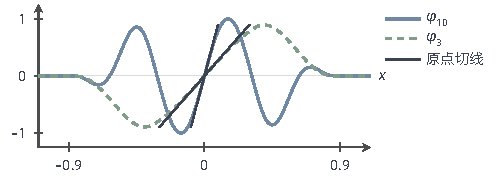
\includegraphics[width=84.4mm]{figures/02-abstract-mathematics/03-function-spaces/tikz/c4-ddelta-test/figure.pdf}
  \caption{区分$D\delta_0$与测度的测试$\varphi_n(x)=\chi(x)\sin(nx)$，$n=3$（虚线）与$n=10$（实线）。两者的支撑都在$[-0.9,0.9]$内，函数值都不超过$1$，测度的读数因而一致有界；原点处的切线斜率却等于$n$，$D\delta_0$的读数$-\varphi_n'(0)=-n$随$n$无界。}
  \label{fig:sob-ddelta-test}
\end{figure}

这个例子与上一小节图~\ref{fig:sob-test-sequences}(b)是同一个机制：只控制函数值不能控制导数的读数。它说明广义函数严格大于测度，求导会把函数（甚至测度）推出原来的对象类型。于是自然要问：从一个局部可积函数出发，它的广义导数什么时候仍然是一个局部可积函数？这正是下一节要回答的问题。
